\section{Mise en Page et Style}
Le style du document est géré par le package \texttt{fancyhdr} pour les en-têtes et pieds de page, et les marges sont définies avec \texttt{geometry}. Assurez-vous que la hauteur de l'en-tête est suffisante pour éviter les avertissements de `fancyhdr`.

\subsection{Figures et Images}
Les figures peuvent être incluses dans le document en utilisant le package \texttt{graphicx}. Voici un exemple d'inclusion d'une figure :

\begin{figure}[!ht]
    \centering
    
\includegraphics[width=0.5\linewidth]{4_attachments/figures/empty_image.png}
    \caption{Exemple d'insertion d'une image}
    \label{fig:empty_image}
\end{figure}

L'environnement `figure` permet de spécifier le positionnement, d'ajouter une légende et de référencer les images dans le texte.

\subsection{Tableaux}
Le tableau suivant présente les formats de fichiers avec leurs caractéristiques. Il utilise le package \texttt{tabularx} pour ajuster automatiquement la largeur des colonnes.

\clearpage

\subsection{Graphiques (TikZ, PGFPlots et Forest)}
Les graphiques peuvent être créés à l'aide de \texttt{tikz} et \texttt{pgfplots}. Voici un exemple de graphique en barres :

\begin{figure}[!ht]
    \centering
    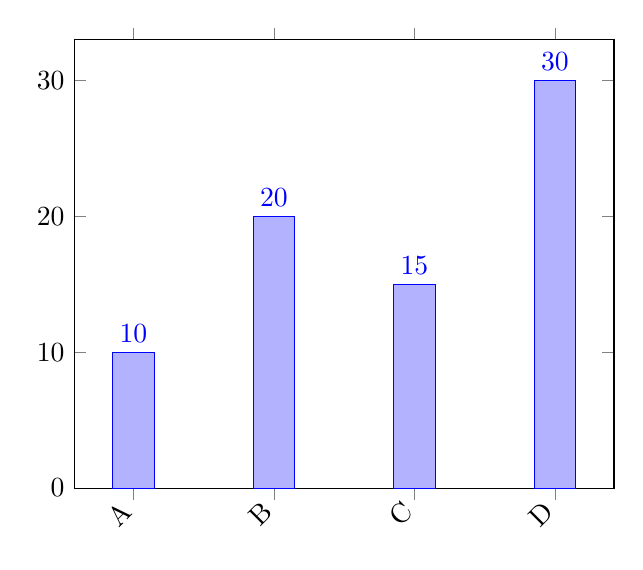
\begin{tikzpicture}
        \begin{axis}[
            ybar,
            symbolic x coords={A, B, C, D},
            xtick=data,
            nodes near coords,
            ymin=0,
            xticklabel style={rotate=45, anchor=east},
            bar width=15pt,
            enlarge x limits={abs=0.75cm},
        ]
        \addplot coordinates {(A, 10) (B, 20) (C, 15) (D, 30)};
        \end{axis}
    \end{tikzpicture}
    \caption{Exemple de graphique en barres}
    \label{fig:graphique}
\end{figure}

Le package \texttt{forest} est utilisé pour créer des diagrammes en arbre. Voici un exemple illustrant la structure du projet :

\begin{figure}[!ht]
    \centering
    \begin{forest}
      for tree={
        grow'=0,
        draw,
        rounded corners,
        node options={align=center, draw, rounded corners},
        fit=band,
        anchor=west,
        parent anchor=east,
        child anchor=west,
        edge path={
          \noexpand\path [draw, \forestoption{edge}]
          (!u.parent anchor) -- +(5pt,0) |- (.child anchor)\forestoption{edge label};
        },
        s sep+=5pt,
        l sep+=10pt,
      }
      [root
        [Branche A
          [Item A.1]
          [Item A.2]
        ]
        [Branche B
          [Item B.1]
          [Item B.2]
        ]
      ]
    \end{forest}
    \caption{Exemple d'arbre avec Forest}
    \label{fig:tree_structure}
\end{figure}